\documentclass[a4paper,10pt,twocolumn,oneside]{article}
\setlength{\columnsep}{10pt}                                                              %兩欄模式的間距
\setlength{\columnseprule}{0pt}                                                                %兩欄模式間格線粗細

\usepackage{amsthm}								%定義,例題
\usepackage{amssymb}
%\usepackage[margin=2cm]{geometry}
\usepackage{fontspec}								%設定字體
\usepackage{color}
% \usepackage{float}
%\usepackage{subfigure}
\usepackage[x11names]{xcolor}
\usepackage{listings}								%顯示code用的
%\usepackage[Glenn]{fncychap}						%排版,頁面模板
\usepackage{fancyhdr}								%設定頁首頁尾
\usepackage{graphicx}								%Graphic
\usepackage{enumerate}
\usepackage{titlesec}
\usepackage{amsmath}
\usepackage[CheckSingle, CJKmath]{xeCJK}
% \usepackage{CJKulem}
%\usepackage[T1]{fontenc}
\titlespacing{\section}{0cm}{0cm}{0cm}
\titlespacing{\subsection}{0cm}{0cm}{0cm}
\usepackage{amsmath, courier, listings, fancyhdr, graphicx}
\topmargin=0pt
\headsep=5pt
\textheight=780pt
\footskip=0pt
\voffset=-40pt
\textwidth=545pt
\marginparsep=0pt
\marginparwidth=0pt
\marginparpush=0pt
\oddsidemargin=0pt
\evensidemargin=0pt
\hoffset=-42pt

%\renewcommand\listfigurename{圖目錄}
%\renewcommand\listtablename{表目錄} 

%%%%%%%%%%%%%%%%%%%%%%%%%%%%%

\setmainfont{Consolas}				%主要字型
\setmonofont{Monaco}				%主要字型
\setCJKmainfont{Noto Sans TC}
%\setCJKmainfont{Consolas}			%中文字型
%\setmainfont{sourcecodepro}
\XeTeXlinebreaklocale "zh"						%中文自動換行
\XeTeXlinebreakskip = 0pt plus 1pt				%設定段落之間的距離
\setcounter{secnumdepth}{3}						%目錄顯示第三層

%%%%%%%%%%%%%%%%%%%%%%%%%%%%%
\makeatletter
\lst@CCPutMacro\lst@ProcessOther {"2D}{\lst@ttfamily{-{}}{-{}}}
\@empty\z@\@empty
\makeatother
\lstset{											% Code顯示
language=C++,										% the language of the code
basicstyle=\footnotesize\ttfamily, 						% the size of the fonts that are used for the code
%numbers=left,										% where to put the line-numbers
numberstyle=\footnotesize,						% the size of the fonts that are used for the line-numbers
stepnumber=1,										% the step between two line-numbers. If it's 1, each line  will be numbered
numbersep=5pt,										% how far the line-numbers are from the code
backgroundcolor=\color{white},					% choose the background color. You must add \usepackage{color}
showspaces=false,									% show spaces adding particular underscores
showstringspaces=false,							% underline spaces within strings
showtabs=false,									% show tabs within strings adding particular underscores
frame=false,											% adds a frame around the code
tabsize=2,											% sets default tabsize to 2 spaces
captionpos=b,										% sets the caption-position to bottom
breaklines=true,									% sets automatic line breaking
breakatwhitespace=false,							% sets if automatic breaks should only happen at whitespace
escapeinside={\%*}{*)},							% if you want to add a comment within your code
morekeywords={*},									% if you want to add more keywords to the set
keywordstyle=\bfseries\color{Blue1},
commentstyle=\itshape\color{Red4},
stringstyle=\itshape\color{Green4},
}
\begin{document}

%%%%%%%%%%%%%%%%%%%%%%%%%%%%%%%%%%%%%%%
\pagestyle{fancy}
\fancyfoot{}
%\fancyfoot[R]{\includegraphics[width=20pt]{ironwood.jpg}}
\fancyhead[L]{National Taiwan Ocean University Physics Mid-term Exam}
\fancyhead[R]{Made By Mr.JB \thepage}
\renewcommand{\headrulewidth}{0.4pt}
%\renewcommand{\contentsname}{Contents} 

\scriptsize
%\tableofcontents
%%%%%%%%%%%%%%%%%%%%%%%%%%%%%%%%%%%%%%%%%
\setlength{\parindent}{0pt}
\begin{normalsize}

\section{公式}

\subsection{向量}
$|\vec{u}|=\sqrt{\vec{i}^2+\vec{j}^2+\vec{k}^2}$ \quad %長度
$a_{x}=a\cos\theta$ \quad
$b_{x}=b\sin\theta$ \\
$|\hat{u}|=\frac{u}{|\vec{u}|}$ \quad %單位向量
$|\vec{a}\cdot\vec{b}|=|\vec{a}||\vec{b}|\cos\theta$ \\ %內積
$\vec{a}\cdot\vec{b}=a_{x}b_{x}+a_{j}b_{j}+a_{z}b_{z}$ \quad
$\vec{a}\times\vec{b}=|\vec{a}||\vec{b}|\sin\theta$ \\ %外積
$\vec{a}\times\vec{b}=\vec{i}$
\begin{vmatrix}
    a_{2} & a_{3} \\
    b_{2} & b_{3}
\end{vmatrix}
$-\vec{j}$
\begin{vmatrix}
    a_{1} & a_{3} \\
    b_{1} & b_{3}
\end{vmatrix}
$+\vec{k}$
\begin{vmatrix}
    a_{1} & a_{2} \\
    b_{1} & b_{2}
\end{vmatrix}
\\
\subsection{微積分}
$\frac{d}{dx}x_{t}=v_{t}$ \quad
$\frac{d}{dx}v_{t}=a_{t}$ \quad
$\frac{d}{dx}log_{e}|x|=\frac{1}{x}$ \\
$\frac{d}{dx}e^x=e^x$ \quad
$\frac{d}{dx}a^x=a^xlog_{e}a$ \\
$\int v_{t}=x_{t}$ \quad
$\int a_{t}=v_{t}$ \\
$\int \frac{1}{x}dx=log_{e}|x|$ \quad
$\int a^xdx=\frac{a^x}{log_{e}}+c$ \\
$\int e^xdx=e^x$ 


\subsection{靜電力 庫倫定律}
$基本電荷 e=1.602\times10^{-19}C$ \\
$k_{e}=8.99\times 10^9 \frac{N\cdot m^2}{c^2}=\frac{1}{4 \pi \varepsilon_{0}}$ \\
$\varepsilon_{0}=8.85 \times 10^{-12} \frac{C^2}{N\cdot m^2}$ \\
$\vec{F}=k_{e}\frac{q_{1}q_{2}}{r^2}\hat{r}$  $ $
$ \hat{r}表示兩粒子延伸軸單位向量$ \\
$\vec{E}=\frac{\vec{F}}{q}=k_{e}\frac{q_{1}}{r^2}\frac{N}{C}$ \\
\begin{tabular}{|c|c|c|}
    \hline
    電荷&符號&單位 \\
    \hline
    & $q$ & $c$ \\
    \hline
    線電荷密度& $ \lambda $ & $ \frac{C}{m} $ \\
    \hline
    面電荷密度& $ \sigma $ & $ \frac{C}{m^2} $ \\
    \hline
    體電荷密度& $ \varrho $ & $ \frac{C}{m^3} $ \\
    \hline
\end{tabular} \\
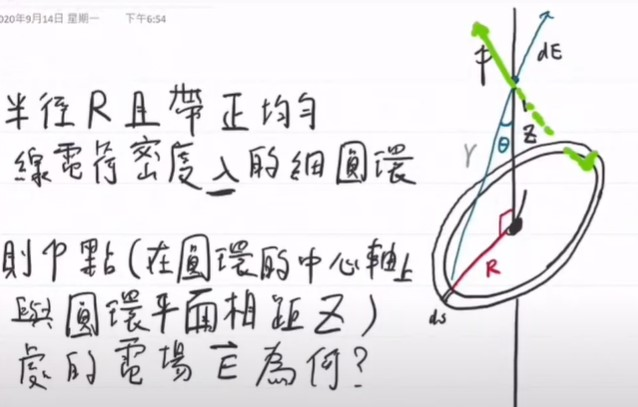
\includegraphics[width=3in]{RingAndCharge.jpg}\\
$dq=\lambda ds$ \\
$dE=\frac{1}{4 \pi \varepsilon_{0}}\frac{dq}{r^2}=\frac{1}{4 \pi \varepsilon_{0}}\frac{\lambda ds}{r^2}=\frac{1}{4 \pi \varepsilon_{0}}\frac{\lambda ds}{Z^2 + R^2}$\\
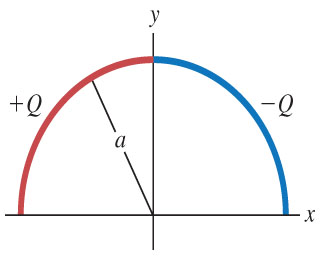
\includegraphics[width=1in]{21-98.jpg} 
$ |E|=\frac{4kQ}{\pi a^2} $\\

\subsection{基礎電路}
$I=\frac{Q}{t}=\frac{n \cdot A \cdot L \cdot e}{\frac{L}{V_{d}}}=nA_{e}V_{d}$\\
$ e:載子的單位電量$ $n:每單位體積載子數$\\$A:截面積$ $L:長度$\\
$ V_{t}=E-V_{r} $ \quad $ R=\rho \times \frac{l}{A}$\\ 
$ P=\frac{W}{t}=\frac{V \times Q}{t}=V\times I=\frac{V^2}{R}=I^2 R$ 

串聯電路 \\
$ E=V_{1}+V_{2}+.....+V_{n}$ \quad
$ R_{T}=R_{1}+R_{2}+.....+R_{n}$ \\ 
% 克希荷夫電壓定律 \\
% $ \sum V_{rise}=\sum V_{drop} $ \\
% $ \sum V = \sum V_{rise}-\sum V_{drop} =0$ \\ 
並聯電路 \\
$ E=V_{1}=V_{2}=.....=V_{n}$ \quad
$ I_{n}=\frac{E}{R_{n}}=G_{n}\times E$ \\ 
$ G_{T}=G_{1}+G_{2}+.....+G_{n}$ \\
$ \frac{1}{R_{T}}=\frac{1}{R_{1}}+\frac{1}{R_{2}}+.....+\frac{1}{R_{n}}$ \\ 
% 克希荷夫電流定律 \\
% $ \sum I_{in}=\sum I_{out} $ \\
% $ \sum V = \sum I_{in}-\sum I_{out} =0$ \\
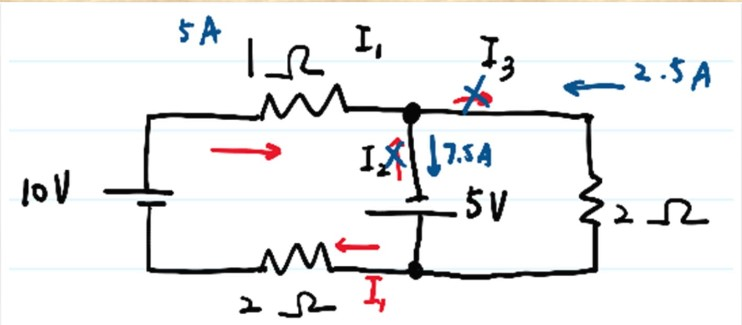
\includegraphics[height=1in]{kirchhoff.jpg}\\
$
\left\{
\begin{array}{l}
Junction \quad  I_{1}+I_{2}=I_{3}\\
左迴路 \quad  10-I_{1}\cdot 1+5-I_{1} \cdot 2 =0\\
右迴路 \quad -2 \cdot I_{3}-5=0
\end{array}
\right .
$ \\
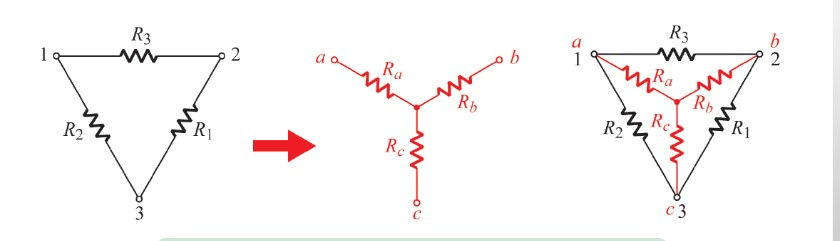
\includegraphics[width=3in]{TriangleCircuit.jpg} \\
$ R_{ab}=\frac{(R_{1}+R_{2} \times R_{3})}{R_{1}+R_{2}+R_{3}}$ \
$ R_{bc}=\frac{(R_{2}+R_{3} \times R_{1})}{R_{1}+R_{2}+R_{3}}$ \
$ R_{ca}=\frac{(R_{3}+R_{1} \times R_{2})}{R_{1}+R_{2}+R_{3}}$ \\
$ R_{a}=\frac{R_{2}R_{3}}{R_{1}+R_{2}+R_{3}}$ \
$ R_{b}=\frac{R_{3}R_{1}}{R_{1}+R_{2}+R_{3}}$ \
$ R_{c}=\frac{R_{1}R_{2}}{R_{1}+R_{2}+R_{3}}$ \\
%$ R_{a}+R_{b}+R_{c}=\frac{(R_{1}R_{2}+R_{2}R_{3}+R_{3}R_{1})}{R_{1}+R_{2}+R_{3}}$\\
$ R_{1}=\frac{R_{a}R_{b}+R_{b}R_{c}+R_{c}R_{a}}{R_{a}}$ \
$ R_{2}=\frac{R_{a}R_{b}+R_{b}R_{c}+R_{c}R_{a}}{R_{b}}$\\
$ R_{3}=\frac{R_{a}R_{b}+R_{b}R_{c}+R_{c}R_{a}}{R_{c}}$\\
惠斯同電橋\\
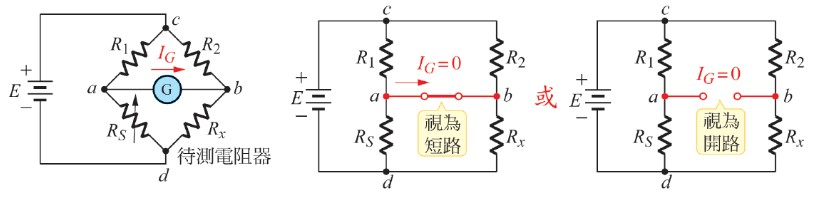
\includegraphics[width=3in]{Wheatstone.jpg}\\
$ R_{2} \times R_{s}=R_{1} \times R_{x} $ \\
電壓表倍增器(倍增率m)(串聯)
$ R_{m}=R_{v}\times (m-1)$\\
電流表分流器(倍增率n)(並聯)
$ R_{s}=\frac{R_{A}}{n-1}$
\subsection{高斯定律}
$ 通量\phi (flux)$
$ \phi=\vec{V} \cdot \vec{A}=V \cdot A \cos \theta$ \\$ V為流速$ $ A為面積向量 $ $\theta 為與\vec{A} 夾角$\\
$ 電場通量\phi$
$\phi=\sum \vec{E} \cdot \varDelta \vec{A} (\frac{N\cdot m^2}{C})\\
高斯定律通過高斯面之總電通量 $\phi$ \\與該曲面之靜電荷 $q_{enc}$ 之間關係 
%$ \varepsilon_{0} \cdot \phi = q_{enc}$\\
$ \phi = \frac{\sum q_{enc}}{\varepsilon_{0}}$ \\
$ 如果q_{enc}為正,淨通量向外$  $如果q_{enc}為負,淨通量向內$\\
$ \phi = \oint \vec{E} \cdot d \vec{A}$\\
$ \phi \varpropto E \varpropto 通過每單位面積電場線數目$\\
Case 1: 球體為導體(R為球半徑)(屏蔽效應)\\
$r \geq R$  $E=\frac{1}{4 \pi \varepsilon_{0}}\frac{q}{r^2}$\\
$r < R$ $E=0$\\
Case 2: 球體為非導體(R為球半徑 $\rho$為體電荷密度)\\
$r > R$ $E=\frac{1}{4 \pi \varepsilon_{0}}\frac{q}{r^2}=\frac{\rho(\frac{4}{3} \pi R^3)}{4 \pi \varepsilon_{0}}\frac{1}{r^2} = \frac{\rho R^3}{3 r^2 \varepsilon_{0}}$\\
$r < R$ $E=\frac{1}{4 \pi \varepsilon_{0}}\frac{q'}{r^2}=\frac{\rho(\frac{4}{3} \pi R^3)\frac{r^3}{R^3}}{4 \pi \varepsilon_{0}}\frac{1}{r^2}=\frac{\rho r}{3\varepsilon_{0}}$\\
$ 高斯轉庫倫$ $E=\frac{1}{4 \pi \varepsilon_{0}}\frac{ q_{enc}}{r^2} $  $F= \frac{1}{4 \pi \varepsilon_{0}} \frac{q \cdot q_{enc}}{r^2} $


\\
\section{翻譯}

\begin{tabular}{|c|c|c|c|c|c|c|c|c|c|c|c|}
    \hline
    \multicolumn{3}{|c|}{electric charge}&\multicolumn{3}{c|}{電荷}&\multicolumn{3}{c|}{electric filed}&\multicolumn{3}{c|}{電場} \\
    \hline
    \multicolumn{6}{|c|}{opposites attract}&\multicolumn{6}{c|}{異性相吸}   \\
    \hline
    \multicolumn{6}{|c|}{likes repel}&\multicolumn{6}{|c|}{同性相斥}\\
    \hline
    \multicolumn{3}{|c|}{conductor}&\multicolumn{3}{c|}{導體}&\multicolumn{3}{c|}{insulator}&\multicolumn{3}{c|}{非導體} \\
    \hline
    \multicolumn{3}{|c|}{semi conductor}&\multicolumn{3}{c|}{半導體}&\multicolumn{3}{c|}{linear charge}&\multicolumn{3}{c|}{線電荷} \\
    \hline
    \multicolumn{3}{|c|}{surface charge}&\multicolumn{3}{c|}{面電荷}&\multicolumn{3}{c|}{volume charge}&\multicolumn{3}{c|}{體電荷} \\
    \hline
    \multicolumn{6}{|c|}{electromotive force/emf}&\multicolumn{6}{c|}{電動勢$ \varepsilon $}   \\
    \hline
    \multicolumn{6}{|c|}{voltage drop}&\multicolumn{6}{c|}{電壓降}\\
    \hline
    \multicolumn{6}{|c|}{terminal voltage}&\multicolumn{6}{c|}{端電壓}\\
    \hline
    \multicolumn{2}{|c|}{node}&\multicolumn{2}{|c|}{節點}&\multicolumn{2}{|c|}{branch}&\multicolumn{2}{|c|}{支路}&
    \multicolumn{2}{|c|}{loop}&\multicolumn{2}{|c|}{迴路}\\
    \hline
    \multicolumn{3}{|c|}{mesh}&\multicolumn{3}{c|}{網目}&\multicolumn{3}{|c|}{multiplier}&\multicolumn{3}{c|}{倍增器}\\
    \hline
    \multicolumn{6}{|c|}{series circuit}&\multicolumn{6}{c|}{串聯電路}\\
    \hline
    \multicolumn{6}{|c|}{parallel circuit}&\multicolumn{6}{c|}{並聯電路}   \\
    \hline
    \multicolumn{3}{|c|}{flux}&\multicolumn{3}{c|}{通量}&\multicolumn{3}{|c|}{electric flux}&\multicolumn{3}{c|}{電場通量}\\
    \hline
\end{tabular}
\end{narmalsize}

\begin{small} 

\lstinputlisting{die.cpp}
\end{small}
\end{document}